\documentclass{standalone}
\usepackage{tikz}
\usetikzlibrary{patterns, positioning}


\begin{document}
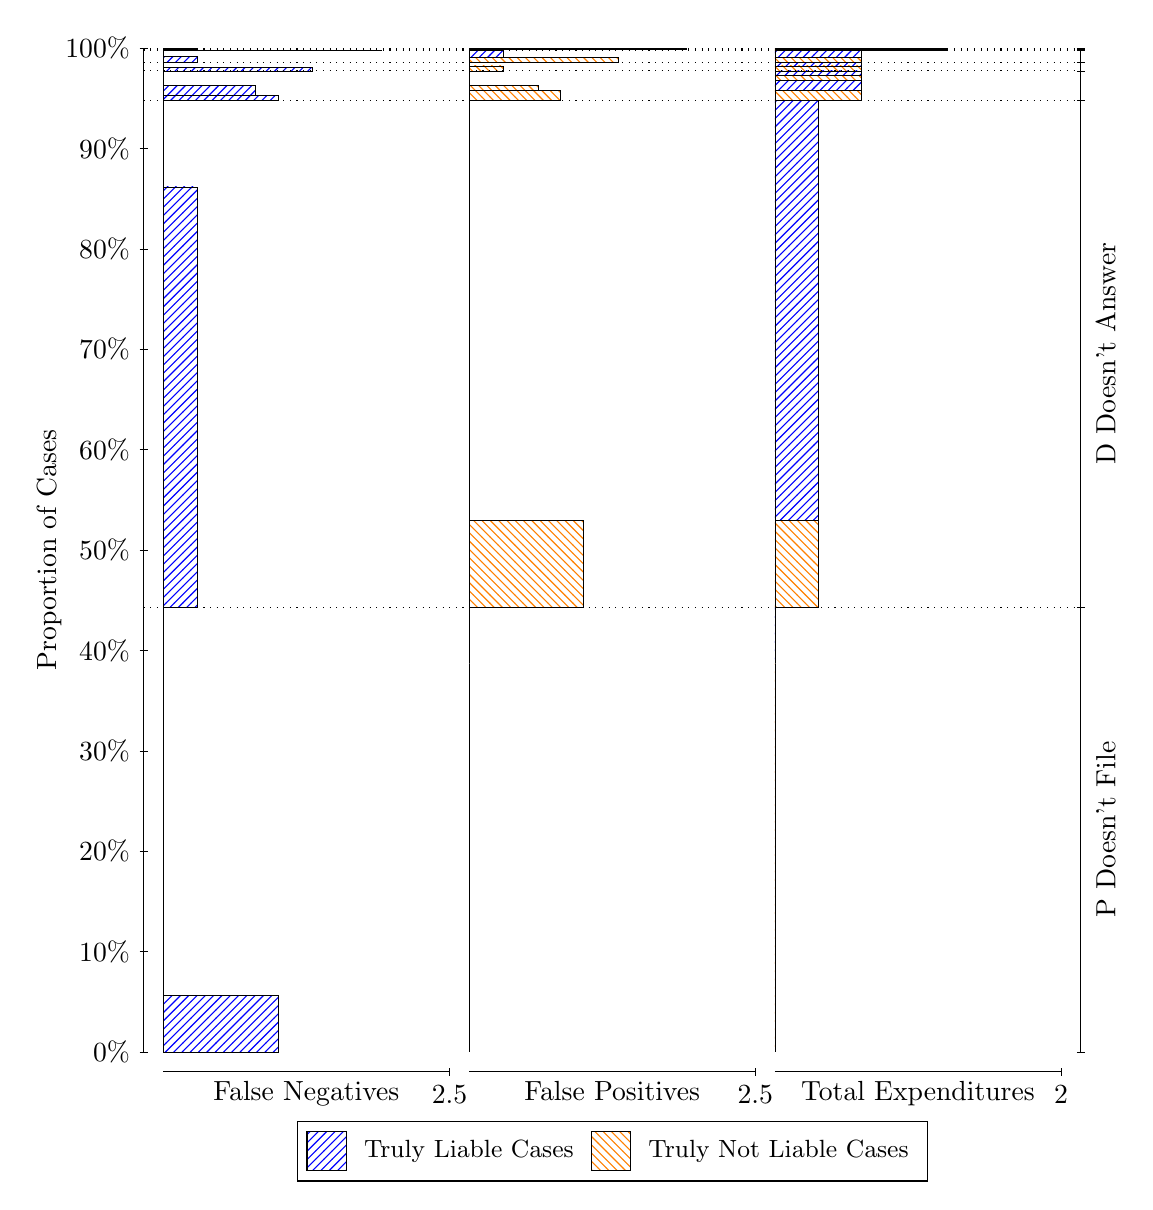
\begin{tikzpicture}
\draw[black, very thin] (1.5,1.75) -- (1.5,14.5);
\node[rotate=90, text=black, anchor=center] at (0.3, 8.125) {Proportion of Cases};
\draw[black, very thin] (1.45,1.75) -- (1.55,1.75);
\node[text=black, anchor=east] at (1.45, 1.75) {0\%};
\draw[black, very thin] (1.45,3.025) -- (1.55,3.025);
\node[text=black, anchor=east] at (1.45, 3.025) {10\%};
\draw[black, very thin] (1.45,4.3) -- (1.55,4.3);
\node[text=black, anchor=east] at (1.45, 4.3) {20\%};
\draw[black, very thin] (1.45,5.575) -- (1.55,5.575);
\node[text=black, anchor=east] at (1.45, 5.575) {30\%};
\draw[black, very thin] (1.45,6.85) -- (1.55,6.85);
\node[text=black, anchor=east] at (1.45, 6.85) {40\%};
\draw[black, very thin] (1.45,8.125) -- (1.55,8.125);
\node[text=black, anchor=east] at (1.45, 8.125) {50\%};
\draw[black, very thin] (1.45,9.4) -- (1.55,9.4);
\node[text=black, anchor=east] at (1.45, 9.4) {60\%};
\draw[black, very thin] (1.45,10.675) -- (1.55,10.675);
\node[text=black, anchor=east] at (1.45, 10.675) {70\%};
\draw[black, very thin] (1.45,11.95) -- (1.55,11.95);
\node[text=black, anchor=east] at (1.45, 11.95) {80\%};
\draw[black, very thin] (1.45,13.225) -- (1.55,13.225);
\node[text=black, anchor=east] at (1.45, 13.225) {90\%};
\draw[black, very thin] (1.45,14.5) -- (1.55,14.5);
\node[text=black, anchor=east] at (1.45, 14.5) {100\%};

\draw[black, very thin] (13.4,1.75) -- (13.4,14.5);
\draw[black, very thin] (13.35,1.75) -- (13.45,1.75);
\node[anchor=west] at (13.35, 1.75) {};
\draw[black, very thin] (13.35,7.4) -- (13.45,7.4);
\node[anchor=west] at (13.35, 7.4) {};
\draw[black, very thin] (13.35,13.838) -- (13.45,13.838);
\node[anchor=west] at (13.35, 13.838) {};
\draw[black, very thin] (13.35,14.209) -- (13.45,14.209);
\node[anchor=west] at (13.35, 14.209) {};
\draw[black, very thin] (13.35,14.317) -- (13.45,14.317);
\node[anchor=west] at (13.35, 14.317) {};
\draw[black, very thin] (13.35,14.467) -- (13.45,14.467);
\node[anchor=west] at (13.35, 14.467) {};
\draw[black, very thin] (13.35,14.488) -- (13.45,14.488);
\node[anchor=west] at (13.35, 14.488) {};
\draw[black, very thin] (13.35,14.5) -- (13.45,14.5);
\node[anchor=west] at (13.35, 14.5) {};

\draw[black, very thin, pattern color=blue, pattern=north east lines] (1.75,1.75) rectangle (3.2033,2.4654);
\draw[black, very thin, pattern color=orange, pattern=north west lines] (1.75,2.4654) rectangle (1.75,7.4);
\draw[black, very thin, pattern color=blue, pattern=north east lines] (1.75,7.4) rectangle (2.186,12.736);
\draw[black, very thin, pattern color=orange, pattern=north west lines] (1.75,12.736) rectangle (1.75,13.838);
\draw[black, very thin, pattern color=blue, pattern=north east lines] (1.75,13.838) rectangle (3.2033,13.898);
\draw[black, very thin, pattern color=blue, pattern=north east lines] (1.75,13.898) rectangle (2.9127,14.023);
\draw[black, very thin, pattern color=orange, pattern=north west lines] (1.75,14.023) rectangle (1.75,14.209);
\draw[black, very thin, pattern color=blue, pattern=north east lines] (1.75,14.209) rectangle (3.6393,14.252);
\draw[black, very thin, pattern color=orange, pattern=north west lines] (1.75,14.252) rectangle (1.75,14.317);
\draw[black, very thin, pattern color=blue, pattern=north east lines] (1.75,14.317) rectangle (2.186,14.398);
\draw[black, very thin, pattern color=orange, pattern=north west lines] (1.75,14.398) rectangle (1.75,14.467);
\draw[black, very thin, pattern color=blue, pattern=north east lines] (1.75,14.467) rectangle (4.5113,14.473);
\draw[black, very thin, pattern color=orange, pattern=north west lines] (1.75,14.473) rectangle (1.75,14.488);
\draw[black, very thin, pattern color=blue, pattern=north east lines] (1.75,14.488) rectangle (2.186,14.495);
\draw[black, very thin, pattern color=orange, pattern=north west lines] (1.75,14.495) rectangle (1.75,14.5);
\draw[black, very thin, pattern color=orange, pattern=north west lines] (5.6333,1.75) rectangle (5.6333,6.6846);
\draw[black, very thin, pattern color=blue, pattern=north east lines] (5.6333,6.6846) rectangle (5.6333,7.4);
\draw[black, very thin, pattern color=orange, pattern=north west lines] (5.6333,7.4) rectangle (7.0867,8.5021);
\draw[black, very thin, pattern color=blue, pattern=north east lines] (5.6333,8.5021) rectangle (5.6333,13.838);
\draw[black, very thin, pattern color=orange, pattern=north west lines] (5.6333,13.838) rectangle (6.796,13.963);
\draw[black, very thin, pattern color=orange, pattern=north west lines] (5.6333,13.963) rectangle (6.5053,14.023);
\draw[black, very thin, pattern color=blue, pattern=north east lines] (5.6333,14.023) rectangle (5.6333,14.209);
\draw[black, very thin, pattern color=orange, pattern=north west lines] (5.6333,14.209) rectangle (6.0693,14.273);
\draw[black, very thin, pattern color=blue, pattern=north east lines] (5.6333,14.273) rectangle (5.6333,14.317);
\draw[black, very thin, pattern color=orange, pattern=north west lines] (5.6333,14.317) rectangle (7.5227,14.385);
\draw[black, very thin, pattern color=blue, pattern=north east lines] (5.6333,14.385) rectangle (6.0693,14.467);
\draw[black, very thin, pattern color=orange, pattern=north west lines] (5.6333,14.467) rectangle (6.0693,14.482);
\draw[black, very thin, pattern color=blue, pattern=north east lines] (5.6333,14.482) rectangle (5.6333,14.488);
\draw[black, very thin, pattern color=orange, pattern=north west lines] (5.6333,14.488) rectangle (8.3947,14.493);
\draw[black, very thin, pattern color=blue, pattern=north east lines] (5.6333,14.493) rectangle (6.9413,14.5);
\draw[black, very thin, pattern color=orange, pattern=north west lines] (9.5167,1.75) rectangle (9.5167,6.6846);
\draw[black, very thin, pattern color=blue, pattern=north east lines] (9.5167,6.6846) rectangle (9.5167,7.4);
\draw[black, very thin, pattern color=orange, pattern=north west lines] (9.5167,7.4) rectangle (10.062,8.5021);
\draw[black, very thin, pattern color=blue, pattern=north east lines] (9.5167,8.5021) rectangle (10.062,13.838);
\draw[black, very thin, pattern color=orange, pattern=north west lines] (9.5167,13.838) rectangle (10.607,13.963);
\draw[black, very thin, pattern color=blue, pattern=north east lines] (9.5167,13.963) rectangle (10.607,14.088);
\draw[black, very thin, pattern color=orange, pattern=north west lines] (9.5167,14.088) rectangle (10.607,14.149);
\draw[black, very thin, pattern color=blue, pattern=north east lines] (9.5167,14.149) rectangle (10.607,14.209);
\draw[black, very thin, pattern color=orange, pattern=north west lines] (9.5167,14.209) rectangle (10.607,14.273);
\draw[black, very thin, pattern color=blue, pattern=north east lines] (9.5167,14.273) rectangle (10.607,14.317);
\draw[black, very thin, pattern color=orange, pattern=north west lines] (9.5167,14.317) rectangle (10.607,14.385);
\draw[black, very thin, pattern color=blue, pattern=north east lines] (9.5167,14.385) rectangle (10.607,14.467);
\draw[black, very thin, pattern color=orange, pattern=north west lines] (9.5167,14.467) rectangle (11.697,14.482);
\draw[black, very thin, pattern color=blue, pattern=north east lines] (9.5167,14.482) rectangle (11.697,14.488);
\draw[black, very thin, pattern color=orange, pattern=north west lines] (9.5167,14.488) rectangle (11.697,14.493);
\draw[black, very thin, pattern color=blue, pattern=north east lines] (9.5167,14.493) rectangle (11.697,14.5);
\draw[black, dotted] (1.5,7.4) -- (13.4,7.4);
\draw[black, dotted] (1.5,13.838) -- (13.4,13.838);
\draw[black, dotted] (1.5,14.209) -- (13.4,14.209);
\draw[black, dotted] (1.5,14.317) -- (13.4,14.317);
\draw[black, dotted] (1.5,14.467) -- (13.4,14.467);
\draw[black, dotted] (1.5,14.488) -- (13.4,14.488);
\draw[black, very thin] (1.75,1.5) -- (5.3833,1.5);
\node[text=black, anchor=north] at (3.5667, 1.5) {False Negatives};
\draw[black, very thin] (5.3833,1.45) -- (5.3833,1.55);
\node[text=black, anchor=north] at (5.3833, 1.45) {2.5};

\draw[black, very thin] (5.6333,1.5) -- (9.2667,1.5);
\node[text=black, anchor=north] at (7.45, 1.5) {False Positives};
\draw[black, very thin] (9.2667,1.45) -- (9.2667,1.55);
\node[text=black, anchor=north] at (9.2667, 1.45) {2.5};

\draw[black, very thin] (9.5167,1.5) -- (13.15,1.5);
\node[text=black, anchor=north] at (11.333, 1.5) {Total Expenditures};
\draw[black, very thin] (13.15,1.45) -- (13.15,1.55);
\node[text=black, anchor=north] at (13.15, 1.45) {2};

\node[text=black, centered, rotate=90] at (13.72, 4.575) {P Doesn't File};
\node[text=black, centered, rotate=90] at (13.72, 10.619) {D Doesn't Answer};






\draw (7.449999999999999,1.5) node[draw=none] (baseCoordinate) {};
\begin{scope}[align=center]
        \matrix[scale=0.5, draw=black, below=0.5cm of baseCoordinate, nodes={draw}, column sep=0.1cm]{
            \node[rectangle, draw, minimum width=0.5cm, minimum height=0.5cm, pattern color=blue, pattern=north east lines] {}; &
            \node[draw=none, font=\small, text=black] (B) {Truly Liable Cases}; &
            \node[rectangle, draw, minimum width=0.5cm, minimum height=0.5cm, pattern color=orange, pattern=north west lines] {}; &
            \node[draw=none, font=\small, text=black] (B) {Truly Not Liable Cases}; \\
            };
\end{scope}

\end{tikzpicture}
\end{document}